\documentclass{article}
\usepackage{pgfplots}
\pgfplotsset{compat=1.18}

\begin{document}

\begin{figure}[h]
\centering
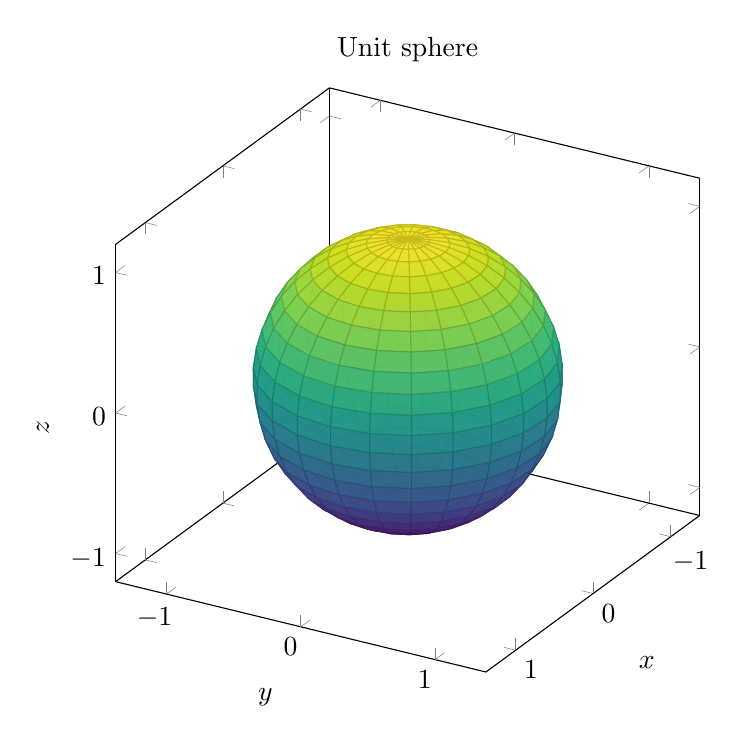
\begin{tikzpicture}
\begin{axis}[
    axis equal,
    width=9cm, height=9cm,
    view={120}{25},
    xlabel=$x$, ylabel=$y$, zlabel=$z$,
    colormap name=viridis,
    title={Unit sphere},
]
\addplot3[
    surf,
    z buffer=sort,
    opacity=0.9,
    samples=24,
    domain=0:360,
    y domain=0:180,
    point meta=z,
] (
    {cos(x)*sin(y)},
    {sin(x)*sin(y)},
    {cos(y)}
);
\end{axis}
\end{tikzpicture}
\caption{The unit sphere parametrised by azimuth and polar angle.}
\end{figure}

\end{document}
